\documentclass[12pt]{article}
\usepackage{parskip}
\usepackage[letterpaper, margin=1in]{geometry}
\usepackage{graphicx}
\usepackage{amsmath}
\graphicspath{{./images/}}
\title{ELECENG 2EI5 Lab 2}
\author{Raeed Hassan \\ hassam41 \\  \\ McMaster University}
\begin{document}
\maketitle
\pagebreak

\section*{The Minimum}
\begin{enumerate}
    \item The IV-characteristics of the 1N5225B zener diode included in our 2EI5 parts kit is shown in Figure 1.
    \begin{figure}[h!]
        \centering
        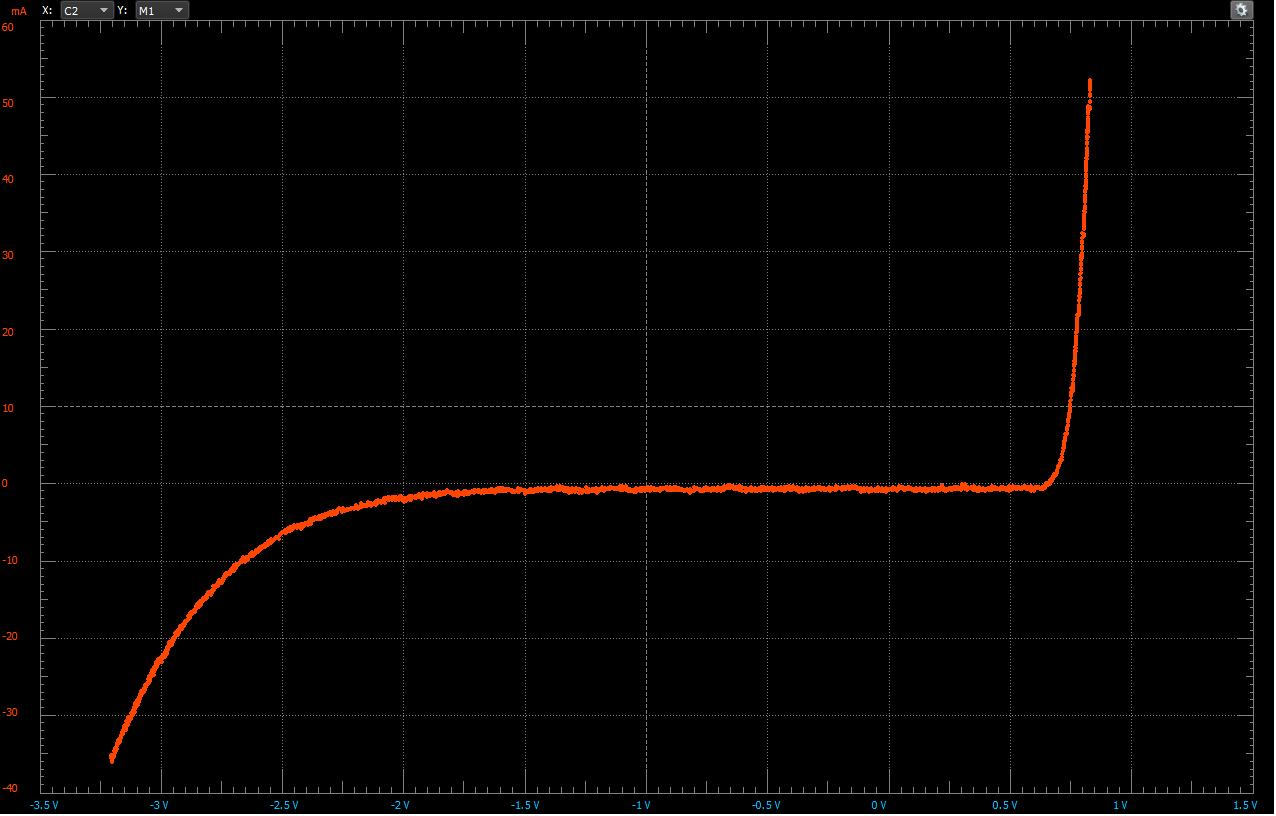
\includegraphics[width=0.7\textwidth]{A1.png}
        \caption{IV-characteristics of 1N5225B zener diode}
    \end{figure}
    \item A photograph of the circuit setup used to produce the IV-characteristics in Figure 1 is shown in Figure 2.
    \begin{figure}[h!]
        \centering
        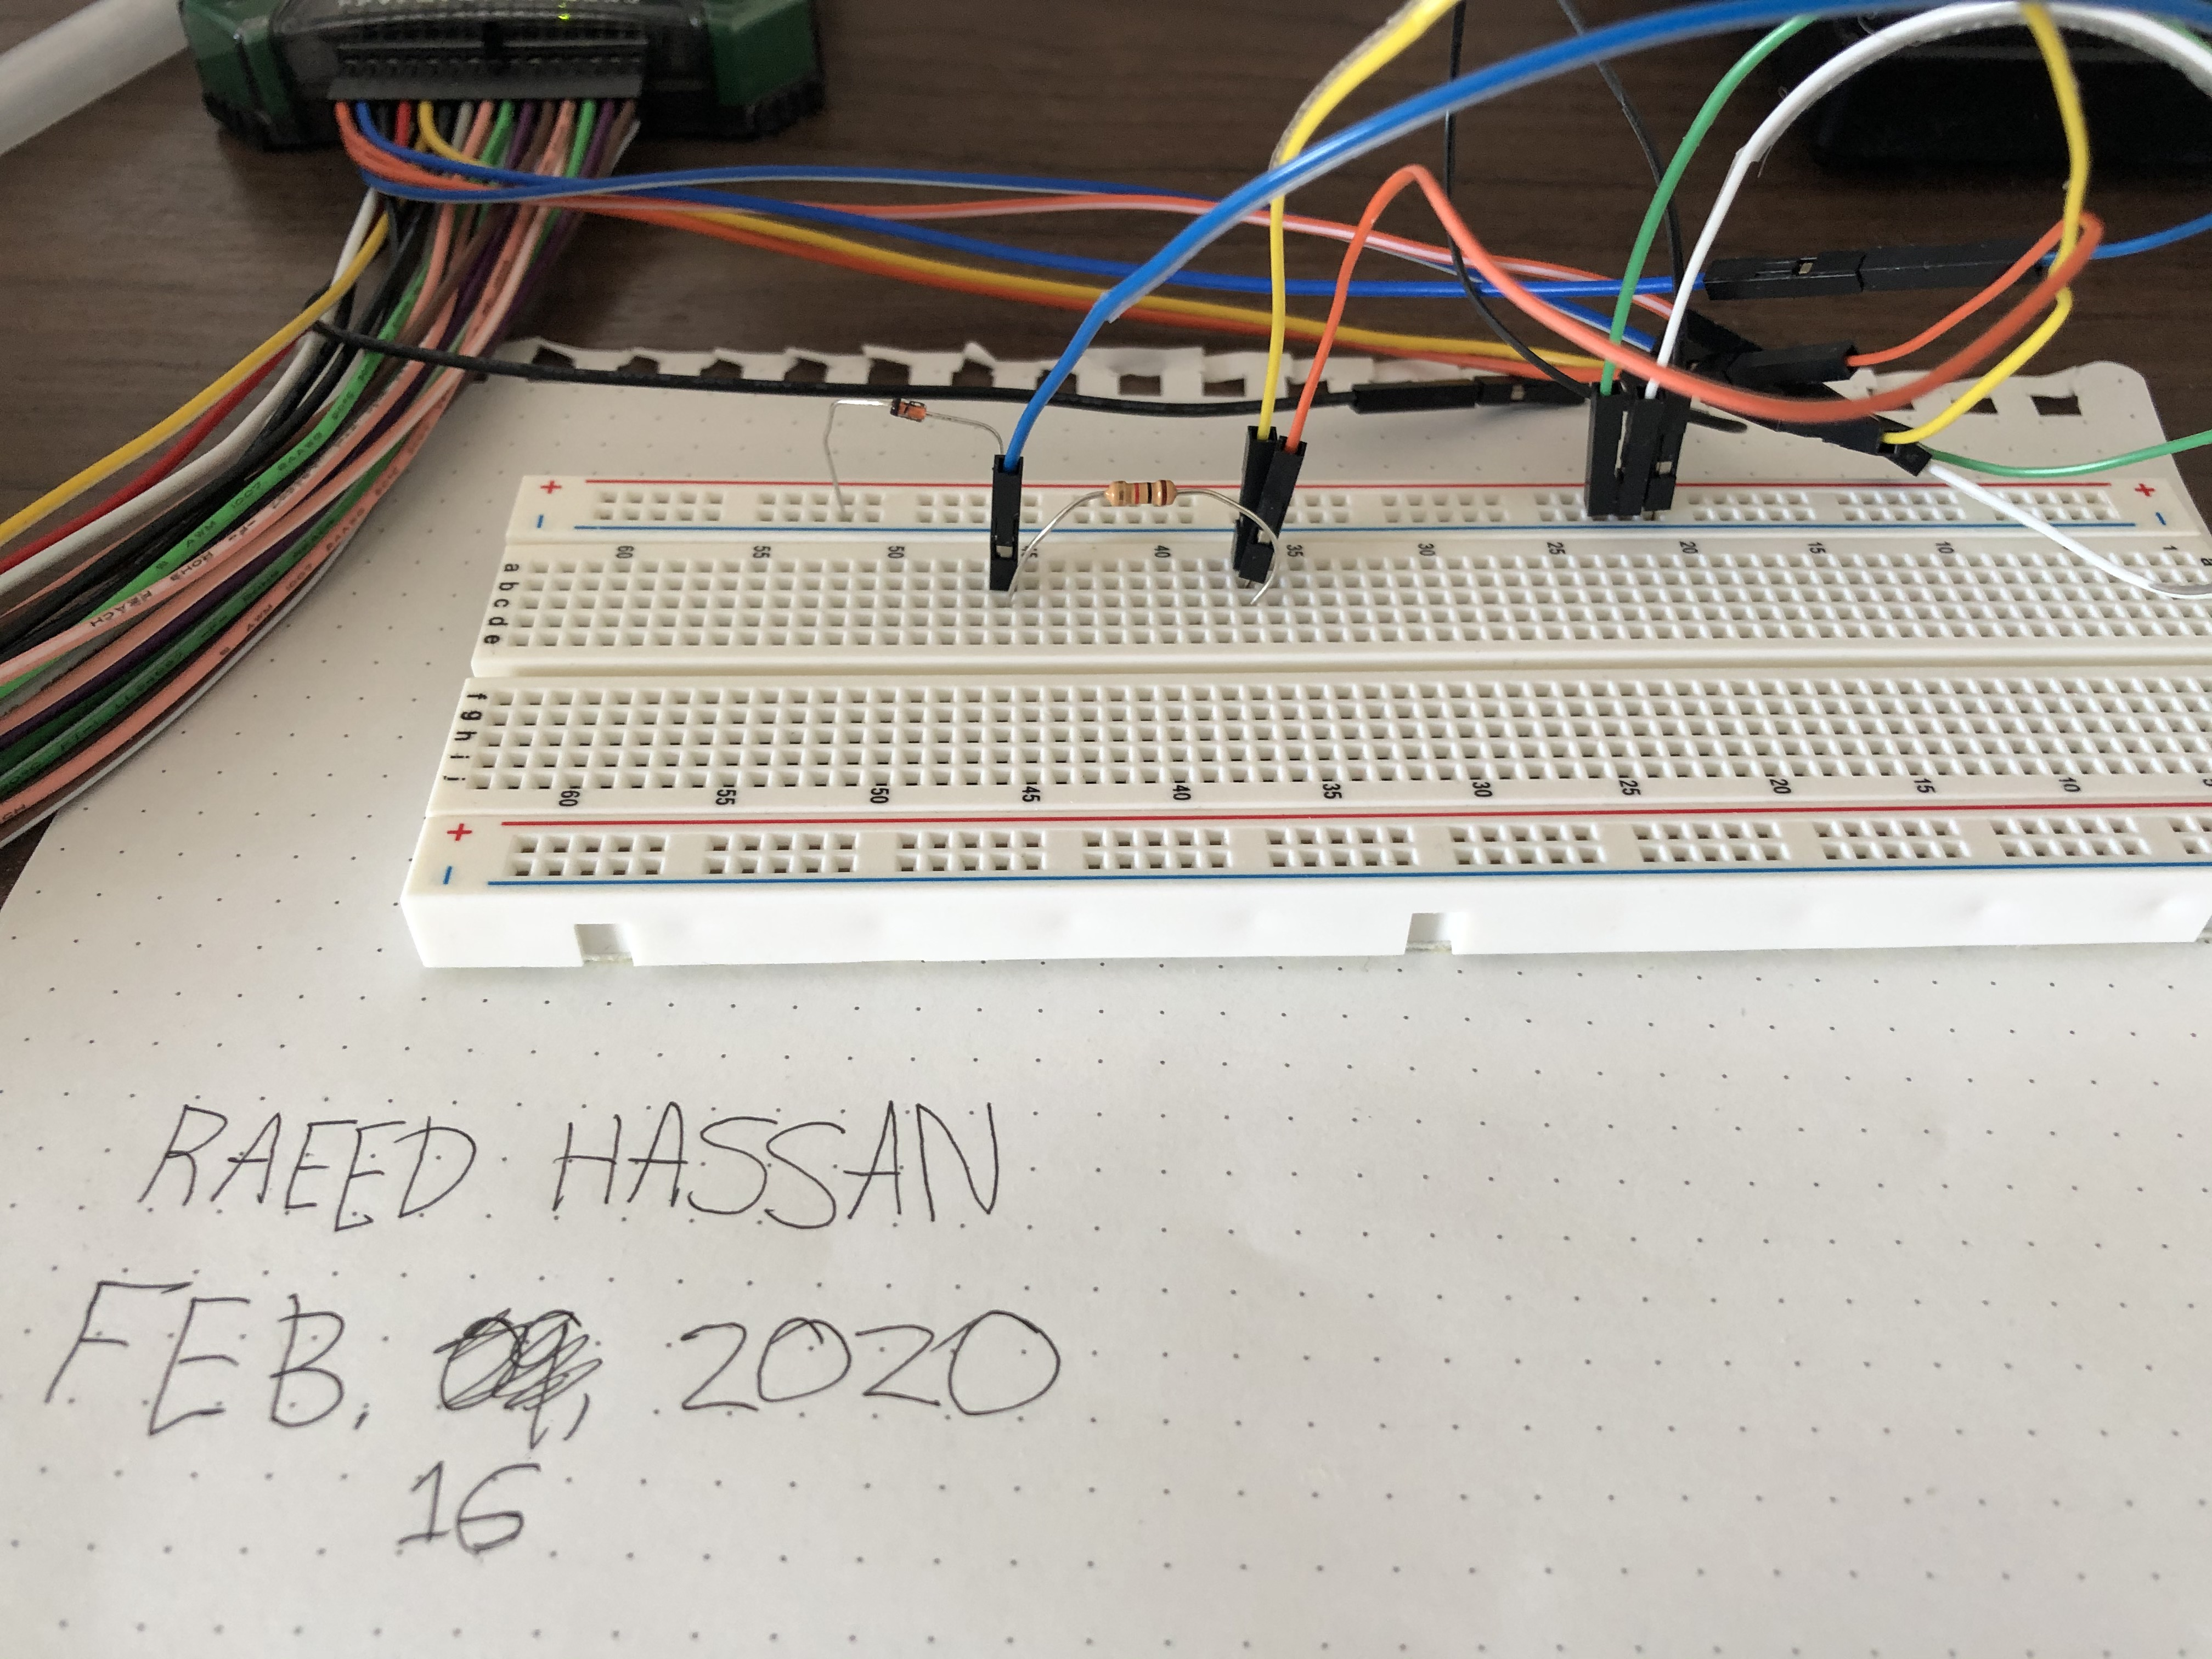
\includegraphics[width=0.7\textwidth]{A2.png}
        \caption{Photograph of circuit setup}
    \end{figure}
    \item According to the datasheet for the 1N5225B zener diode, the zener breakdown voltage is typically $3V$, with minimum and maximum values being $2.85V$ and $3.15V$. The minimum current required to put the diode in zener breakdown is $20mA$.
    \begin{enumerate}
        \item The measured zener breakdown voltage approximately 2.90V, which is between the typical and minimum rated values for the diode.  
        \item The minimum current required to put the diode in zener breakdown is measured to be approximately 16.5mA, which is slightly less than the value in the datasheet. However, it is expected the current would be slightly less as the zener breakdown voltage is less than the typical value.
    \end{enumerate}
\end{enumerate}

\section*{The Bulk}
\begin{enumerate}
    \item The simulations for the circuit are shown in Figure 3.
    \begin{figure}[h!]
        \centering
        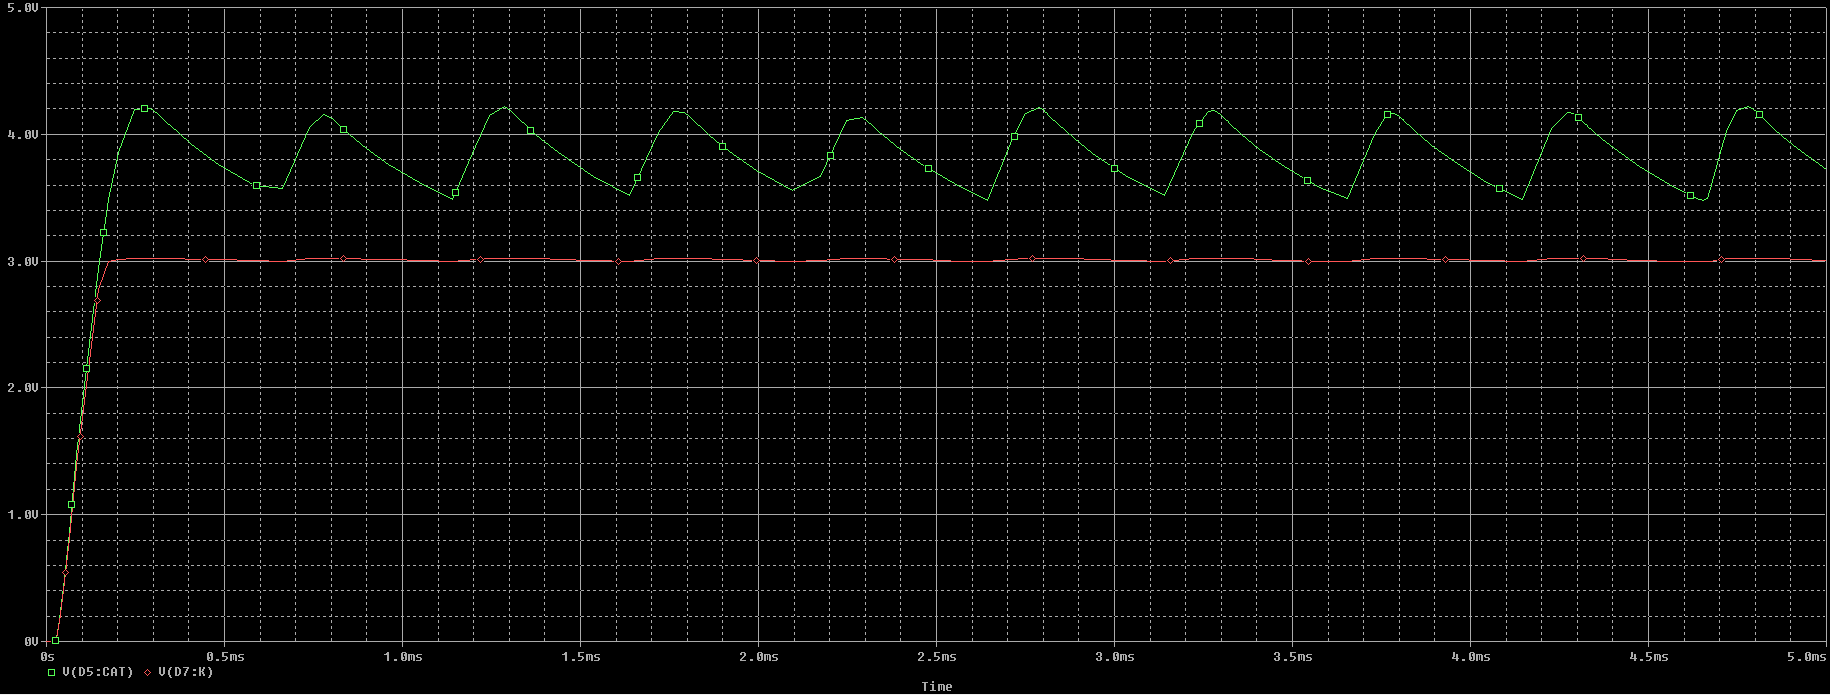
\includegraphics[width=\textwidth]{B1.png}
        \caption{Simulation of $v_c$ (green) and $v_o$ (red).}
    \end{figure}
    \item An increase in R causes a decrease in $v_o$, an increase in $v_c$, and a decrease in the voltage ripple in both $v_c$ and $v_o$, while a decrease in R leave the average value of $v_o$ unchanged but causes a decrease in $v_c$ and an in the voltage ripple in both $v_c$ and $v_o$. The changes in $v_o$ and $v_c$ eventually stop and their values will plateau at a fixed value. An increase in C causes a decrease in the voltage ripple of both $v_c$ and $v_o$, while a decrease in C causes an increase in the voltage ripple of both $v_c$ and $v_o$. Changes in C do not affect the average value of $v_o$ or $v_c$, but does increase the time constant of the circuit (increase in C increases time constant, decrease in C decreases time constant).
    \item The voltage plots for $v_c$ and $v_o$ for the circuit built using $R_L = 340\Omega$, $R=20\Omega$, and $C=20\mu F$ is shown in Figure 4. This is the same scenario that was simulated in Figure 1, which was found to have safe current values for the components in the build circuit.
    \begin{figure}[h!]
        \centering
        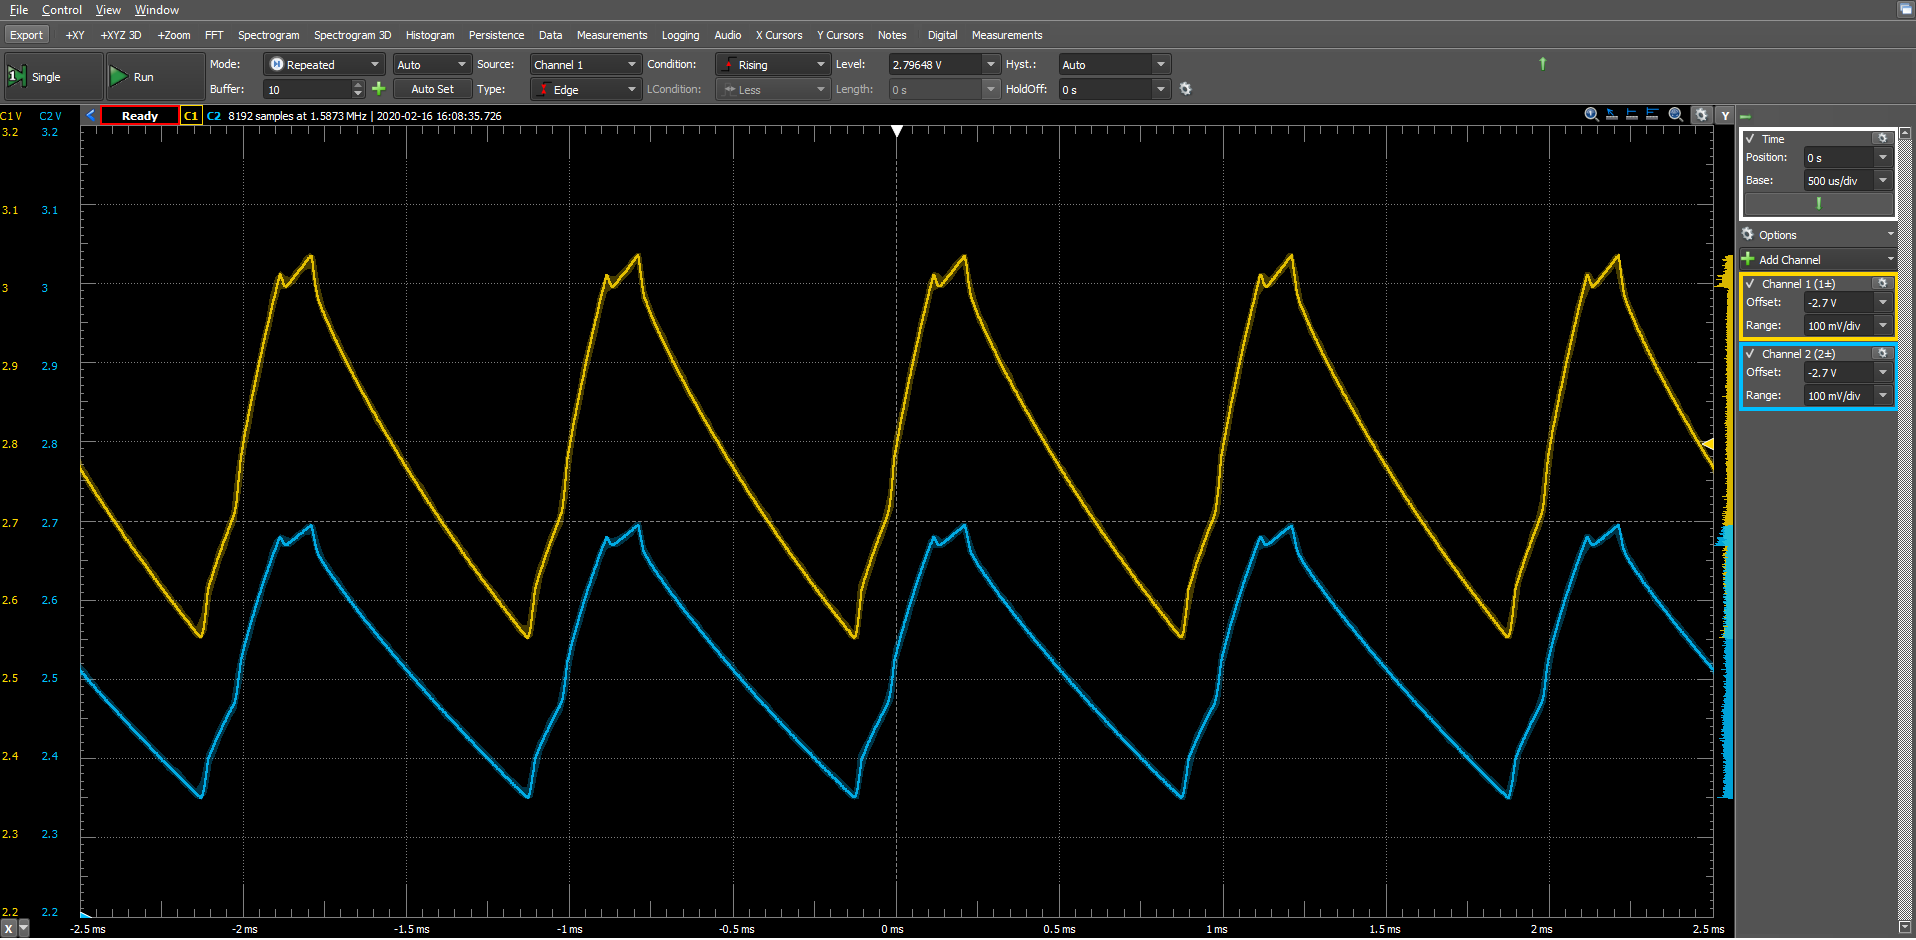
\includegraphics[width=\textwidth]{B2.png}
        \caption{Measurements of $v_c$ (yellow) and $v_o$ (blue).}
    \end{figure}
\end{enumerate}
\pagebreak
\section*{The Max}
The period of the voltage ripple increases substantially when there is only one source present. The voltage ripple also increases with a single source. This result can be seen in Figure 5.
\begin{figure}[h!]
    \centering
    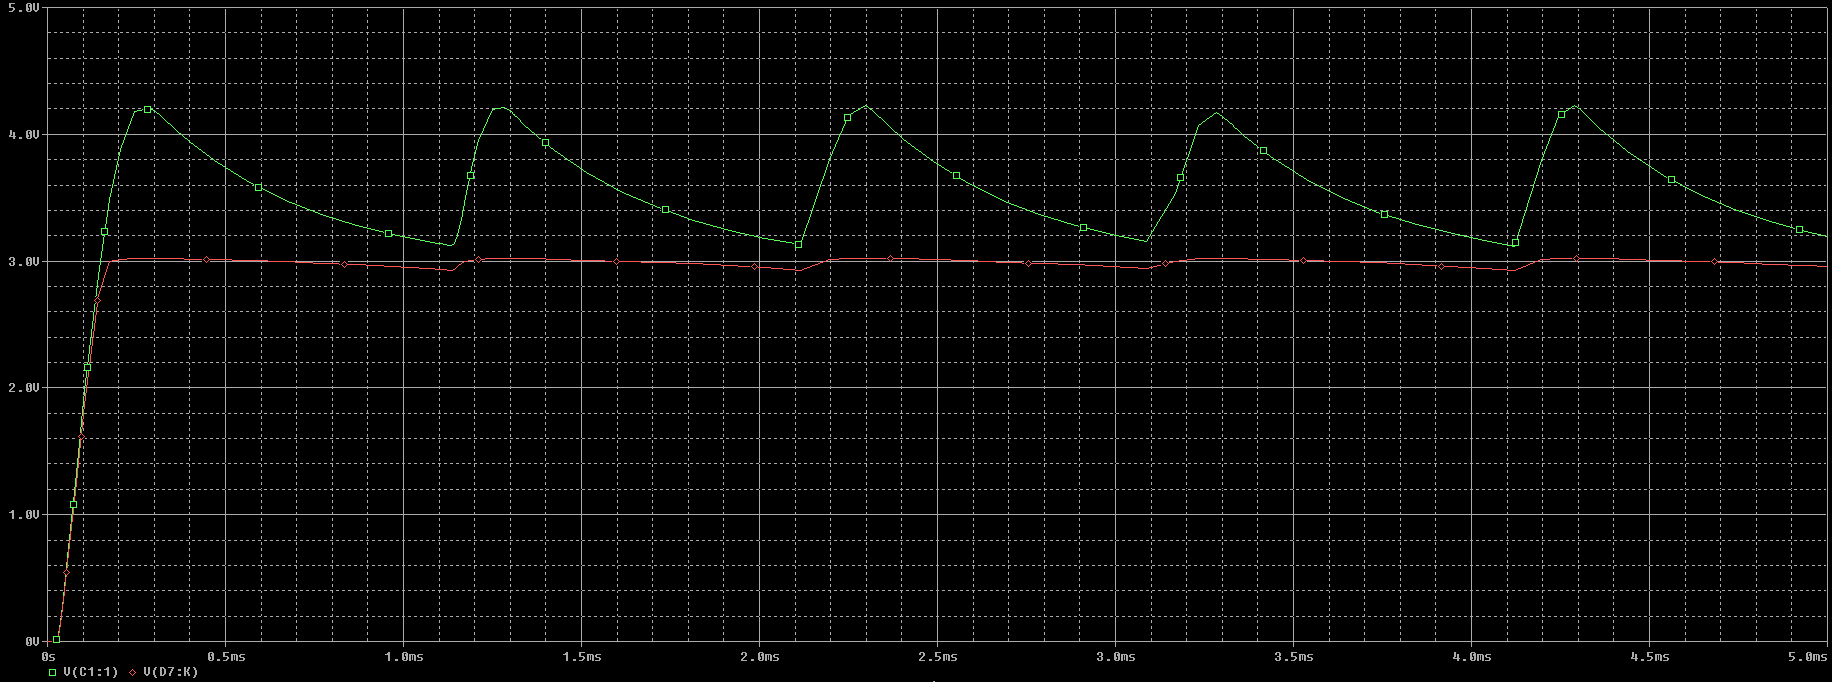
\includegraphics[width=\textwidth]{C1.png}
    \caption{Simulation with single source}
\end{figure} \\
\pagebreak
Increasing the amplitude of the source to 8V causes the average value and the voltage ripple in $v_c$ to increase substantially, however $v_o$ remains largely unchanged. This effect can be seen in Figure 6.
\begin{figure}[h!]
    \centering
    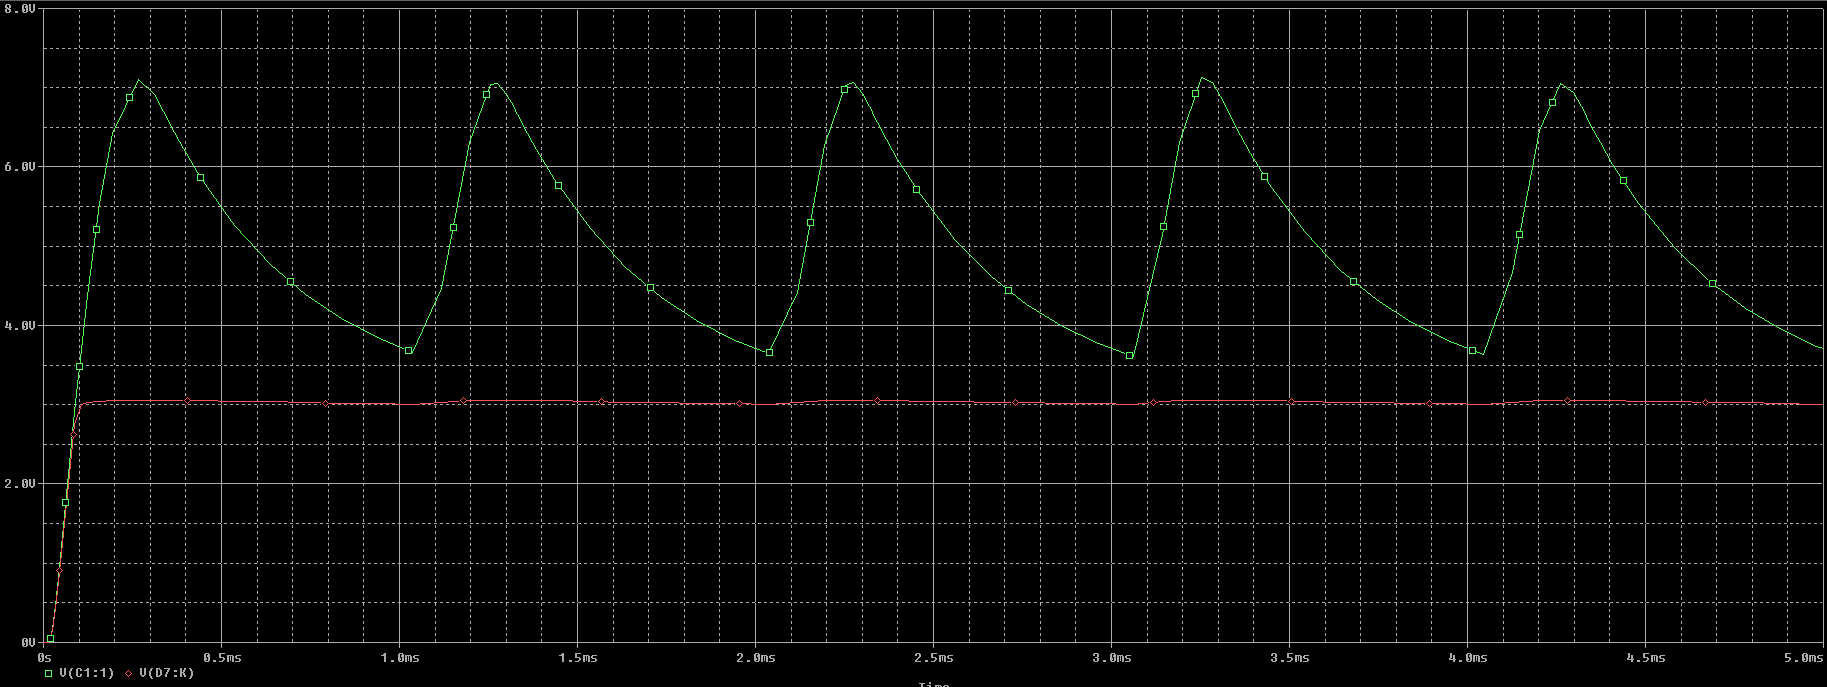
\includegraphics[width=\textwidth]{C2.png}
    \caption{Simulation with source ampltiude at tV}
\end{figure}
\end{document}